\subsection{MFCCs}
Mel Frequency Cepstral Coefficents (MFCCs) are widely used features in ASR and SI. They were introduced by Davis and Mermelstein in the '80s, and have been state-of-the-art ever since.

As the name suggests, MFCCs are based on the Mel-scale (where \textit{Mel} stands for \textit{melody}), a logarithmic scale devised to map the frequency of a sound on a scale that better reflects the human perception of them. Figure \vref{fig:mel_hz_plot} shows the plot of pitch Mel scale versus Hertz scale, we can note how \SI{1000}{mel} equals \SI{1000}{Hz}.

\begin{figure}
	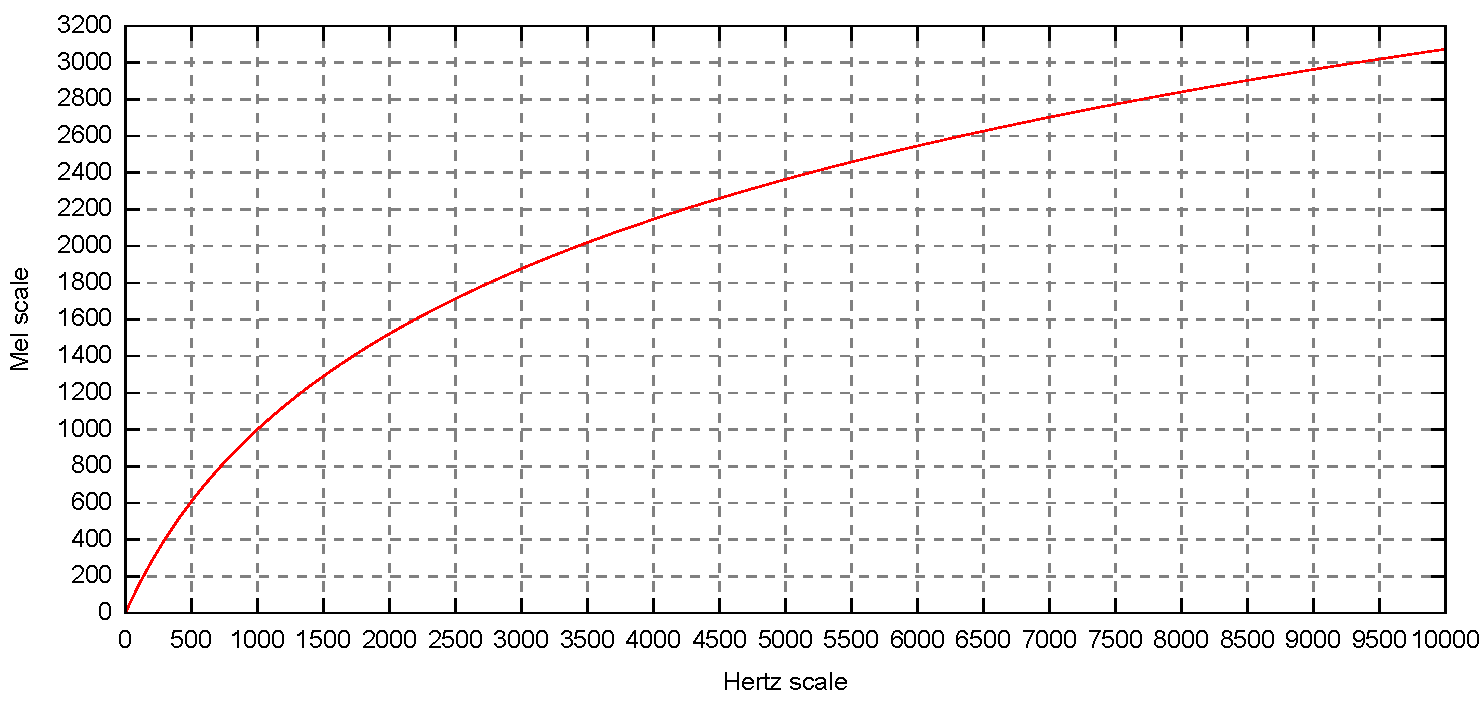
\includegraphics[width=0.5\textwidth]{images/mel_hz_plot}
	\caption{Plot of pitch mel scale versus Hertz scale, source~\cite{wiki:mel_scale}.}
	\label{fig:mel_hz_plot}
\end{figure}

The MFCC feature extraction technique basically includes windowing the signal, applying the DFT, taking the log of the magnitude, and then warping the frequencies on a Mel scale, followed by applying the inverse DCT. The detailed description of the various steps involved in the MFCC feature extraction is explained below.

\subsubsection{Pre-Emphasis}
Pre-emphasis refers to filtering that emphasizes the higher frequencies. It is used to balance the spectrum of voiced sounds that have a steep drop in the high frequency range. Usually the glottal source has a slope of about -12 dB/octave. However, when acoustic energy is radiated from the lips, this results in a spectrum rise of about +6 dB/octave. Therefore, pre-distortion removes some of the glottal effects from the vocal tract parameters.

The most commonly used pre-emphasis filter is given by the following transfer function:
$$
H(z)=1-b z^{-1}
$$

\subsubsection{Framing}
The speech signal is a slowly time-varying or quasi-stationary signal. For stable acoustic characteristics, speech needs to be examined over a sufficiently short period of time. Therefore, speech analysis must always be carried out on short segments across which the speech signal is assumed to be stationary; usually, it is divided into smaller frames each lasting between 20ms and 40ms.

\subsubsection{Windowing}
Advancing the time window every 10 ms enables the temporal characteristics of individual speech sounds to be tracked, and the 20 ms analysis window is usually sufficient to provide good spectral resolution of these sounds, and at the same time short enough to resolve significant temporal characteristics. The purpose of the overlapping analysis is that each speech sound of the input sequence would be approximately centered at some frame. On each frame, a window is applied to taper the signal towards the frame boundaries. This is done to enhance the harmonics, smooth the edges, and to reduce the edge effect while taking the DFT on the signal.
Hamming window has been used as window shape by considering the next block in feature extraction processing chain and integrates all the closest frequency lines. Let:
\begin{itemize}
    \item $X_n$ = input signal;
    \item $Y_n$ = output signal;
    \item $W_n$ = hamming window;
\end{itemize}
then the resulting windowed signal is:
\begin{center}
$Y_n = X_n \times W_n, \quad n=0,1,2,\ldots,N$
\end{center}

\paragraph{DFT Spectrum}
Each windowed frame is converted into magnitude spectrum by applying DFT.
$$
X(k)=\sum_{n=0}^{N-1} x(n) e^{\frac{-j 2 \pi n k}{N}} ; \quad 0 \leq k \leq N-1
$$

\subsubsection{Mel Spectrum}
Mel spectrum is computed by passing the Fourier-transformed signal through a set of band-pass filters known as Mel-filter bank. A Mel is a unit of measure based on the human ears perceived frequency. It does not correspond linearly to the physical frequency of the tone, as the human auditory system apparently does not perceive pitch linearly~\cite{rao:spectral}. We reported the relationship between Mel-scale and Hertz-scale in figure \vref{fig:mel_hz_plot}. The approximation of Mel from physical frequency can be expressed as:
\begin{equation}\label{eq:1}
	f_{\Mel}=2595 \log _{10}\left(1+\frac{f}{700}\right)
\end{equation}
where $f$ denotes the physical frequency in Hz, and $f_{\Mel}$ denotes the perceived frequency~\cite{deller:dt_processing}.

Filter banks can be implemented in either the time domain or the frequency domain, but in MFCC computation, they are usually implemented in the latter one. The center frequencies of the filters are normally evenly spaced on the frequency axis, however, to mimic the perception of the human ear, a warped axis is implemented, according to the nonlinear function given in eq. \vref{eq:1}. The most commonly used filter shaper is triangular, the triangular filter banks with Mel frequency warping we used is presented in figure \vref{fig:mel_filter_bank}.
\begin{figure}
  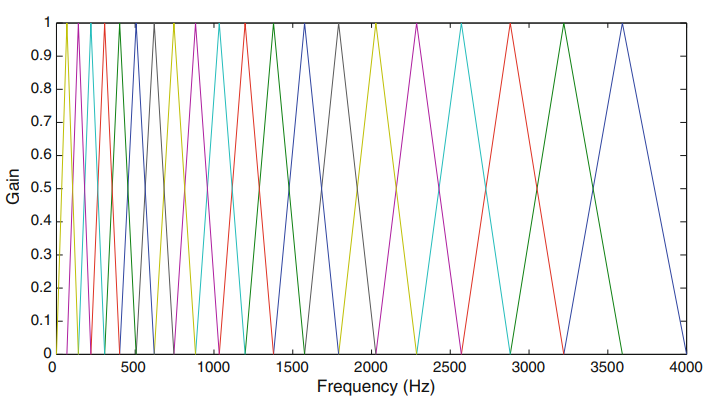
\includegraphics[width=0.5\textwidth]{images/mel_filters.png}
  \caption{Mel-filter bank, source~\cite{rao:spectral}}.
  \label{fig:mel_filter_bank}
\end{figure}

The Mel spectrum of the magnitude spectrum $X(k)$ is computed by multiplying the magnitude spectrum by each of the triangular Mel weighting filters:
\begin{equation}\label{eq:2}
s(m)=\sum_{k=0}^{N-1}\left[ \lvert X(k) \rvert ^{2} H_{m}(k)\right] ; \quad 0 \leq m \leq M-1
\end{equation}
where $M$ is the total number of triangular Mel weighting filters. $H_{m}(k)$ is the weight given to the $k$-th energy spectrum bin contributing to the $m$-th output band and is expressed as~\cite{rao:spectral}:
\begin{equation}
	H_{m}(k)=\left\{\begin{array}{cl}
	0, & k<f(m-1) \\ \\
	\frac{2(k-f(m-1))}{f(m)-f(m-1)}, & f(m-1) \leq k \leq f(m) \\ \\
	\frac{2(f(m+1)-k)}{f(m+1)-f(m)}, & f(m)<k \leq f(m+1) \\ \\
	0, & k>f(m+1)
	\end{array}\right.
\end{equation}

\subsubsection{Discrete Cosine Transform}

Since the vocal tract is smooth, the energy levels in adjacent bands tend to be correlated. Before computing the DCT, the Mel spectrum is usually represented on a log scale, then DCT is applied to the transformed mel frequency coefficients to produce a set of cepstral coefficients. This results in a signal in the cepstral domain with a quefrency peak corresponding to the pitch of the signal and a number of formants representing low quefrency peaks~\cite{rao:spectral}.

Since most of the signal information (corresponding to the vocal tract features) is represented by the first few MFCC coefficients, we only selected the first 13, as usual in most literature. As in~\cite{picone:signal_modeling}, extracting only those coefficients ignoring or truncating higher order DCT components is sufficient to obtain a robust system. Finally we report, again from~\cite{picone:signal_modeling}, the final formula for calculating MFCCs involving DCT:
\begin{equation}
	c(n)=\sum_{m=0}^{M-1} \log _{10}(s(m)) \cos \left(\frac{\pi n(m-0.5)}{M}\right)
\end{equation}
with $n=0,1,2, \ldots, C-1$, where $c(n)$ are the cepstral coefficients and $C$ is the number of MFCCs, usually between \num{8} and \num{13}.

\subsubsection{First and Second Order Derivatives}
First and second derivative of each MFCC (also known as delta and delta-delta features) are also taken into account, since they carry additional information about the coefficient variation over time, ending up with 39 coefficients for each frame, which will become the input of our deep learning model.

Delta coefficients tell about the speech rate, while delta-delta coefficients provide information similar to acceleration of speech~\cite{rao:spectral}. The commonly used definition for computing these dynamic parameters (delta features) is:
\begin{equation}
	\Delta c_m(n) = \frac{\sum_{i = -T}^{T} k_i c_m (n + i)}{\sum_{i = -T}^{T}\lvert i \rvert}
\end{equation}
where $c_m(n)$ denotes the $m$-th feature for the $n$-th time frame, $k_i$ is the $i$-th weight and $T$ is the number of successive frames used for computation. Generally $T$ is taken as $2$. The delta-delta coefficients are computed by taking the first order derivative of the delta coefficients~\cite{rao:spectral}.